\chapter{Layout Recognition For Tabular Data}

To extract elements of a table from an image document, the table first needs to be detected. This is no easy task.  Although for many people, a table is simply a collection of vertical and horizontal lines which can be detected quite easily, this is usually not the case. Often, either the borders are partially or completely missing, the table contains cells of different sizes, multiple columns or rows are merged together on only some places… These and many other factors often cause the table to be of a different form than the well-known matrix. 

Furthermore, complications arise when the image document does not correspond to the typical one-column, graphics-free layout. This often causes complications of reading order and therefore confusing results of text recognition, errors with table detection as spaces between columns can be interpreted as table column borders, and, if tables, forms or other graphic elements are misinterpreted as simple text lines, a text page without any contextual sense. Therefore, in most cases, a \emph{layout analysis} first needs to performed.

\section{Layout Analysis}

\emph{Layout analysis} is the process of identifying and categorizing image document elements, such as figures, tables, forms, math symbols, headers, footers or simple paragraph (\emph{geometric layout analysis}) text and semantically labeling them according to their logical roles (\emph{logical layout analysis}).

In the previous chapter, we already covered the basics of \textbf{geometric layout analysis}, which is the same process as \emph{page segmentation}. The output of this process is a data structure (like vector) containing all of the detected elements. Depending on the configuration of the analysis, the resulting elements can be of various types, such as characters, words, text lines, or even tables and forms. Usually after this, logical layout analysis is applied.

\textbf{Logical layout analysis }is used to determine the reading order of the image document. Its design requires carefully choosing a document structure representation for capturing even the most complex documents. The result of logical layout analysis is often in a form of mapping of each element to its corresponding label. These labels provide an information about the semantical order of the document elements. For example, a label could represent simply the ordering, or it could contain more complex information, such as "table header", "page footer"\ldots

To determine the correct labels is sometimes hard even for a human eye. With various differently aligned columns with different font sizes, or with image captions appearing on different sides of the image in every document, people often determine which elements belong together only according to their intuition (e.g. when reading about a recent earthquake, caption saying “Rescued puppy” probably belongs to the picture of a dog instead of a flooded beach, although in can be placed right in the middle of these two images).

Computer has no notion of such things. This is often a cause of many errors and a reason why a lot of OCR engines claim to work on only documents with specified layouts, e.g. single-column, non-graphical\ldots

\begin{figure}[H]
\centering
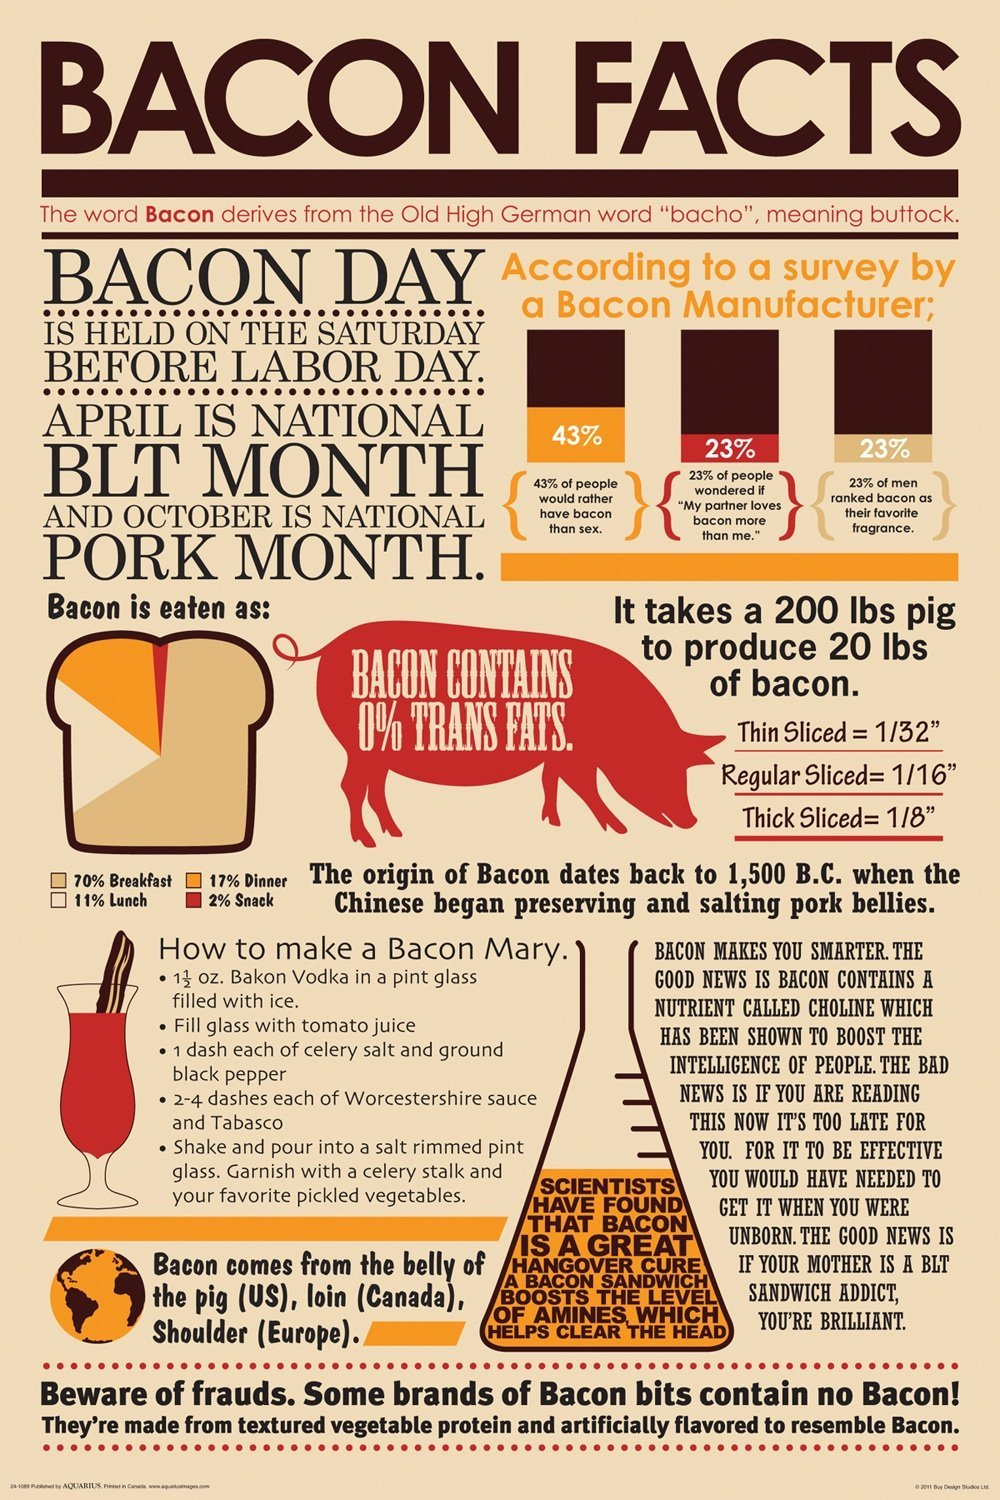
\includegraphics[width=0.5\linewidth]{img/readingOrderIssue.jpg}
\caption{Reading order problems: Determination of correct labels is sometimes hard even for a human eye} \label{fig:1a}
\end{figure}

Various heuristics are being used for determining labels\cite{logicalLayoutTemplate}. In this section, we will be concerned with the few of the most widely used.

\begin{itemize}
\item[\textbf{Templates}] The most simple and basic approach is the technique of the already mentioned templates. It is based on simply mapping the input document to already predefined template, which already has all the information about the structure of elements. Although a naive approach, in the OCR engines used widely for processing a single type of documents (such as ticket validation, recipe or passport recognition, recognition of forms filled out by patients in hospitals), there is no use for anything more complicated, as this process yields almost perfect results.

\item[\textbf{Rule-Based Approaches}] A human reader often determines the logical succession of document elements by font settings and locations of the element. Rule-based approaches take advantage of this fact and create heuristic \emph{rules} that determine the type of the element. For example, a rule for a page header could be "has the smallest y-axis value, has font size above 22pt, is bold, and is the only element on its line".

\item[\textbf{Syntactic Methods}] In this approach, the structure used for element labeling is in the form of a set of formal (usually context free) grammars. These grammars contain rules for aggregating pixels into more and more structured entities until they form logical objects. From these grammars, parsers for the syntactic analysis are automatically obtained. They are then used to perform the actual labeling of the detected elements.

\item[\textbf{Machine Learning}] Already mentioned in this thesis, machine learning methods are widely popular among document recognition. For logical ordering, these methods are even more powerful --- given enough information, the network determines the labeling on its own, without the need of complicated heuristics. However, neural networks need to be trained. This is where different types of machine learning techniques are distinguished. For example, the neural network can be given a set of rules and input images, which leads the learning process closer to the results similar to the human observation. Also, it can be solely reliant on raw physical data and itself.

\end{itemize}

Worth mentioning are also techniques like \emph{Blackboard system} or \emph{Description language} or methods based on \emph{Hidden Markov Models} \cite{logicalLayoutOther}.

Layout analysis is a crucial part of almost every OCR engine. If either geometric or logical analysis fails, the OCR engine will have corrupted input data, which will lead to significantly lower accuracy of the recognition process. 

In this thesis, we focus only on table recognition. Our concern is not the headings and fonts, headers and footers of the image, but only the tabular data. However, this does not mean that layout analysis is unnecessary. We still need to extract the tables from page layout and ideally include also their headers, footers or any other information the table may be containing.

\begin{figure}[H]
\centering
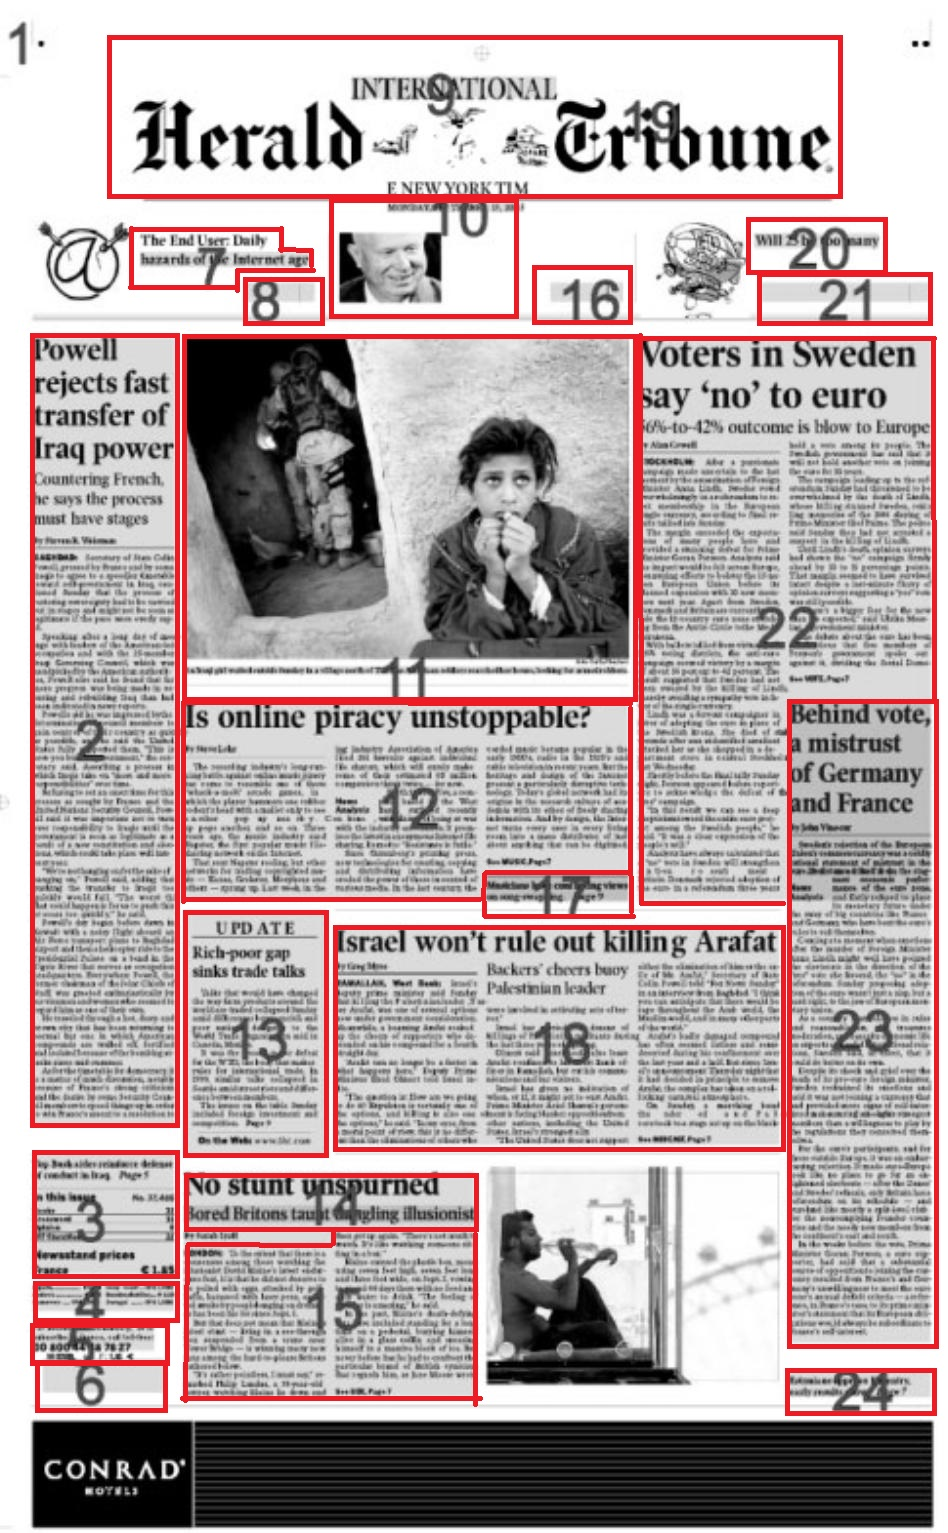
\includegraphics[width=0.5\linewidth]{img/readingOrder.jpg}
\caption{An example of layout analysis \citep{hadjar2004xed}} \label{fig:1a}
\end{figure}

\section{Table Recognition}

The goal of table recognition is to determine if a table even is present on the page, and if yes, where and what its contents are. It is often divided into two parts --- \emph{table detection} and \emph{table decomposition}, with table detection determining the presence and placement of the table, and table decomposition analyzing the contents of the table and presenting a meaningful structure.

However, table detection often greatly depends on the decomposed structure of the table and usually works with it. For example, a table can be detected in the following way:

\begin{enumerate}
    \item find the individual lines (\emph{table decomposition})
    \item check which lines are aligned in a similar way (\emph{table detection})
    \item declare these lines to be in the same table (\emph{table decomposition})
    \item find different columns from the lines (\emph{table decomposition})
\end{enumerate}

If we were to first perform table detection and only then proceed to table decomposition, we would lose the important information about lines that we already obtained in step one. Therefore, many algorithms perform the table recognition process as a whole, which is also the case of our implementation \xxx{mozno taggnut implementaciu?}).

The problem of table detection is challenging due to variable layouts and random positioning of table elements. A basic table (like the default MS Word table) having a default grid layout, with multiple perpendicular horizontal and vertical lines, is not that hard to detect. Its borders could be detected by a simple line detection algorithm (for example Hough transform). However, there are many problems that can complicate this process, like invisible borders, invisible lines, different cell sizes, multiple merged cells..

In this chapter, we will overview some of the already existing table recognition algorithms. We will especially focus on the table recognition implementation of the Tesseract engine, as it is based on the same character recognition as our implementation (\xxx{taggnut results? impl? mozno nejako povedat ze s tymto to budem porovnavat? neviem ako to napisat}). 

\begin{figure}[H]
\centering
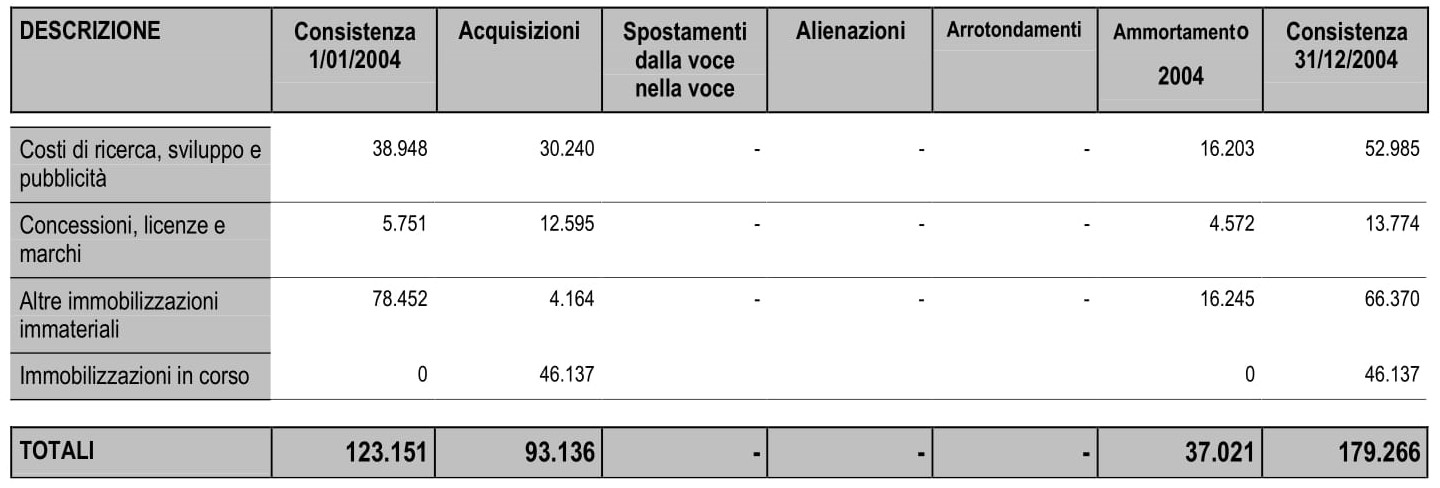
\includegraphics[width=0.7\linewidth]{img/recognitionProblematic.jpg}
\caption{A few of the basic problems with table recognition: missing horizontal and vertical lines; missing information in cells; multiline cells in the first column and header row; different alignment of header and content cells } \label{fig:1a}
\end{figure}

\subsection{Tesseract Table Recognition}

Tesseract is a growing open-source project that was originally used for solely character detection. Over the years, however, it has grown and as of this day, contains various other feature, including a table recognition algorithm.

This algorithm was presented by \citet{tableDetHeterogeneous} and is now part of the software. It is based on already existing Tesseract's features, including layout analysis \xxx{taggnut tie tab-stopy ktore som zmienila hore} and character detection. In this section, we will provide a brief overview of the algorithm, including its advantages and setbacks.

\xxx{popis algorithmu - ako spravim nejako rozumne tie steps?}

Steps of the algorithm include the following: 

\begin{enumerate}
\item \emph{Layout analysis}

Layout analysis is performed by \emph{tab-stop detection} that is already included in the Tesseract library. We already mentioned this method in \xxx{taggnut to hore}. However, the result of this step is not only a list of segmented blocks. For the purposes of the algorithm, this step also saves the column layout and column partitions (sequences of connected components of the same type --- like text, image --- that do not cross any tab-line). The reason for this is the support for multi-column documents.

\item \emph{Column partition analysis}

The information about column layout and column partitions is next used to determine whether the column partition lies completely in one page column, or spans across multiple page columns. Analysis of column partition presence in table regions shows two major scenarios --- in the first case, table columns are reported as page columns, thereby destroying the columnar structure of a page. In the second case, table columns are ignored.

\item \emph{Identifying table partitions}

The next step is to identify text column partitions that could possibly belong to a table --- \emph{table partitions}. This is done based on heuristics, identifying partitions that have at least one large gap, consist of only one word, or overlap with other partitions along the y-axis.

This stage of the algorithm is performed quite aggressively, so although this process returns the desired table partitions, it also produces a lot of false alarms, like section headings, page headers, footers, equations and so on. A smoothing filter is applied to remove these unwanted partitions.

\item \emph{Detecting table columns}

Vertically aligned partitions are simply grouped into a single column with further removal of columns with only one partition. This step pays a close attention to the page layout itself and tries to prevent merging two distinct columns, which is often an issue in full-page tables.

\item \emph{Creating tables}

The goal of the last step is to group table columns into a table. From the assumption that a flowing text does not share space with a table along the y-axis, boundaries of table columns are expanded to the page columns that contain them. Therefore the within column table regions for each page column are obtained. When it comes to tables that span across multiple page columns, these are detected only if a table column exists that belong to both of these page columns.

\item \emph{Removal of false positives}

As the algorithm works quite aggressively, it produces a lot of false positives. Therefore, this step analyzes tables with only one column and removes those that do not suffice certain x-axis projection conditions.

\end{enumerate}

Results of this algorithm have shown 86\% precision. The biggest problems have shown to be full-page tables, often resulting in over or under-segmentation, partial detection or false positive detection. We will further present the results of this algorithm on our data in \xxx{taggni results sekciu}, where we compare them to our algorithm.
   
\begin{figure}[H]
\hspace*{\fill} % separation between the subfigures
\begin{subfigure}{0.31\textwidth}
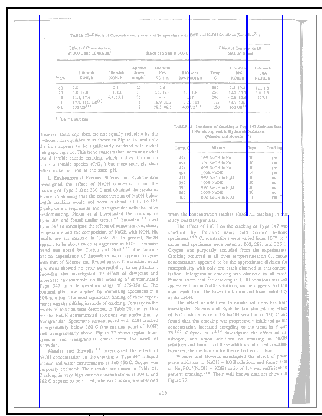
\includegraphics[width=\linewidth]{img/tableDetectionColumns.pdf}
\caption{Column Layout} \label{fig:1a}
\end{subfigure}
\hspace*{\fill} % separation between the subfigures
\begin{subfigure}{0.31\textwidth}
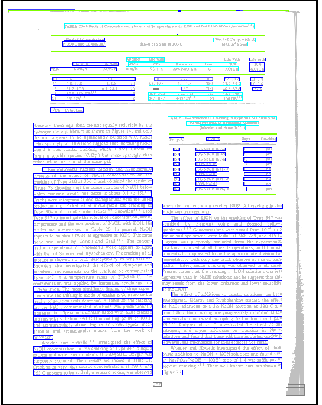
\includegraphics[width=\linewidth]{img/tableDetectionPartitions.pdf}
\caption{Column Partitions} \label{fig:1b}
\end{subfigure}
\hspace*{\fill} % separation between the subfigures
\begin{subfigure}{0.31\textwidth}
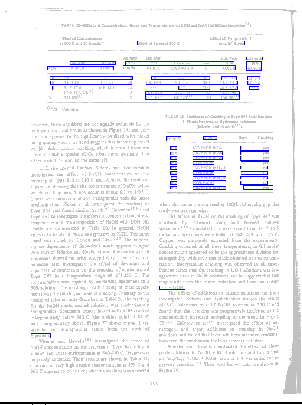
\includegraphics[width=\linewidth]{img/tableDetectionCandidate.pdf}
\caption{Candidate Table Partitions} \label{fig:1c}
\end{subfigure}
\begin{subfigure}{0.31\textwidth}
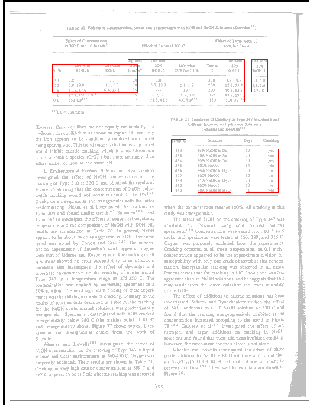
\includegraphics[width=\linewidth]{img/tableDetectionTabCols.pdf}
\caption{Table Columns} \label{fig:1c}
\end{subfigure}
\hspace*{\fill} % separation between the subfigures
\begin{subfigure}{0.31\textwidth}
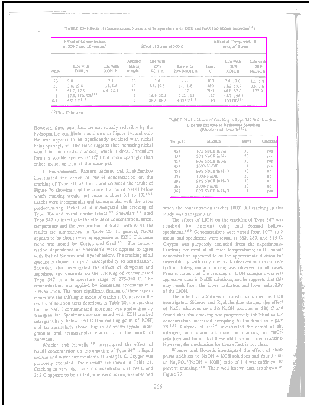
\includegraphics[width=\linewidth]{img/tableDetectionResult.pdf}
\caption{Detected Table Regions} \label{fig:1c}
\end{subfigure}

\caption{The process of Tesseract table recognition} \label{fig:1}
\end{figure}

\subsection{Other existing approaches}

Over the years, there have been many heuristic approaches presented for table detection. In this chapter, we are going to have a look at a few of them and determine what they have in common, as well as point out their pros and cons.

Presented as one of the first table detection algorithms by \citet{TRecs}, the \textbf{T-Recs} table recognition system is based on a bottom-up approach of clustering word bounding boxes and building a "segmentation graph". This results in creating different regions of page, and these are then evaluated according to certain criterion. If they satisfy them, the region is determined to be a table. Although widely used in the future, this techniques has a few setbacks. T-Recs is controlled by a set of numerical parameters, which result in different results of table detection depending on the layout that is given. These parameters need to be set manually. Moreover, it yields unsatisfactory results on multi-column documents.

Another algorithm was described by \citet{MediumTable}. In single-column documents, a page can be easily segmented into individual text-lines. The table detection problem is then perceived as an optimization problem, where the start and end text-lines belonging to a table are identified by optimizing some quality function. However, this approach fails on multi-column documents, or on documents having more than one table.

Problems during analysis of multi-column documents were approached by \citet{tableDetHeterogeneous}. Here, page segmentation process is performed by Tesseract via \emph{tab-stop detection} \xxx{odkaz na section hore?}, which claims to work well on multi-columned documents. Based on the results of Tesseract's analysis, this algorithm then aggressively searches for text column partitions that could possibly belong to a table region. Although this process returns the desired table partitions, it also produces a lot of false alarms, like section headings, page headers, footers, equations and so on. A smoothing filter is applied to remove these unwanted partitions.

Detection of table columns is performed from these partitions. Vertically aligned partitions are simply grouped into a single column with further removal of columns with only one partition. Table columns then need to be grouped together to form a table. In this algorithm, a merge is performed only if at least one horizontal ruling is present between two columns.

Results of this algorithm have shown 86\% precision. The biggest problems have shown to be full-page tables, often resulting in over or under-segmentation, partial detection or false positive detection. 

\citet{tableDetectCesarini} describes another approach based on the document being hierarchically represented by a structure similar to a MXY tree. The presence of a table is determined by searching the tree for parallel lines, which contain white spaces and other perpendicular lines between them. Located tables can be merged on the basis of proximity and similarity criteria. However, this approach fails if no lines in tables are presented --- which is usually the case of many tables.

Another method is presented by \textbf{pdf2table} project \cite{pdf2table}. This method is based on assigning each text object of the page its positional attributes. Depending on them, text objects are then merged into single-lines (lines with only one text object), multi-lines (lines with more than one text object) and multi-line blocks (multiple multi-lines merged together). The table detection algorithm is based on merging multi-line blocks that may belong to the same table, with the help of a heuristical threshold that determines the greatest number of single-line objects between two multi-line blocks possible.

This method also assumes the input to be a single-column documents. However, a user can provide it with an information about the number of columns, which yields much more accurate results.

Multiple other approaches exist, each one of them working on different types of tables and yielding slightly different results. Worth mentioning is, for example, \emph{Sparse Line Detection} \cite{sparseLineDetection}, which however already uses principles based on machine learning. Some of the other methods briefly mentioned by \citet{otherDetection1} or \citet{otherDetection2}.
